\section{Application Acceleration}
\label{sec:acceleration}

In this section, we demonstrate the performance and benefits of the FlashBoost
architecture by presenting some simple accelerator examples. 

\subsection{Nearest Neighbor Search}

Nearest neighbor search is a classical problem with many applications. One of
the modern achievements in this field is Locality Sensitive Hashing~\cite{lsh}.
LSH hashes the dataset using multiple hash functions, so that
similar data is statistically likely to be hashed to similar buckets. When
querying, the query is hashed using the same hash functions, and only the data
in the matching buckets are actually compared. The bulk of the work during a
query process is traversing hash buckets and reading the corresponding data to
perform distance calculation. Because data pointed to by the hash buckets are
most likely scattered across the dataset, access patterns are quite random.

We have built a LSH query accelerator, where all of the data is stored in flash
and the distance calculation is done by the in-storage processor on the storage
device. For simplicity, we assume 8KB data items, and calculate the hamming
distance between the query data and each of the items in the has bucket. The
software sends a stream of addresses from a hash bucket along with the query
data, and the system will return the index of the item most closely matching the
query. By offloading computation to the in-storage accelerator, we
show XXX\% performance improvement over the non-accelerated implementation.



\subsection{Graph Traversal}

Efficient graph traversal is a very important component of any graph processing
system. It is also a very latency-bound problem because one often cannot predict
the next node to visit, until the previous node is visited and processed. We
demonstrate the performance benefits of our FlashBoost architecture by
implementing graph traversal that takes advantages of the in-storage processor
and the integrated storage network, which allows extremely low-latency access
into both local and remote flash storage. The difference latency has on graph
traversal queries can be seen in Figure~\ref{fig:graph_accel}. We demonstrate that compared to a
naive implementation that uses flash only as a storage device, we have XXX\%
performance improvement.

%\begin{figure}[h]
%	\begin{center}
%	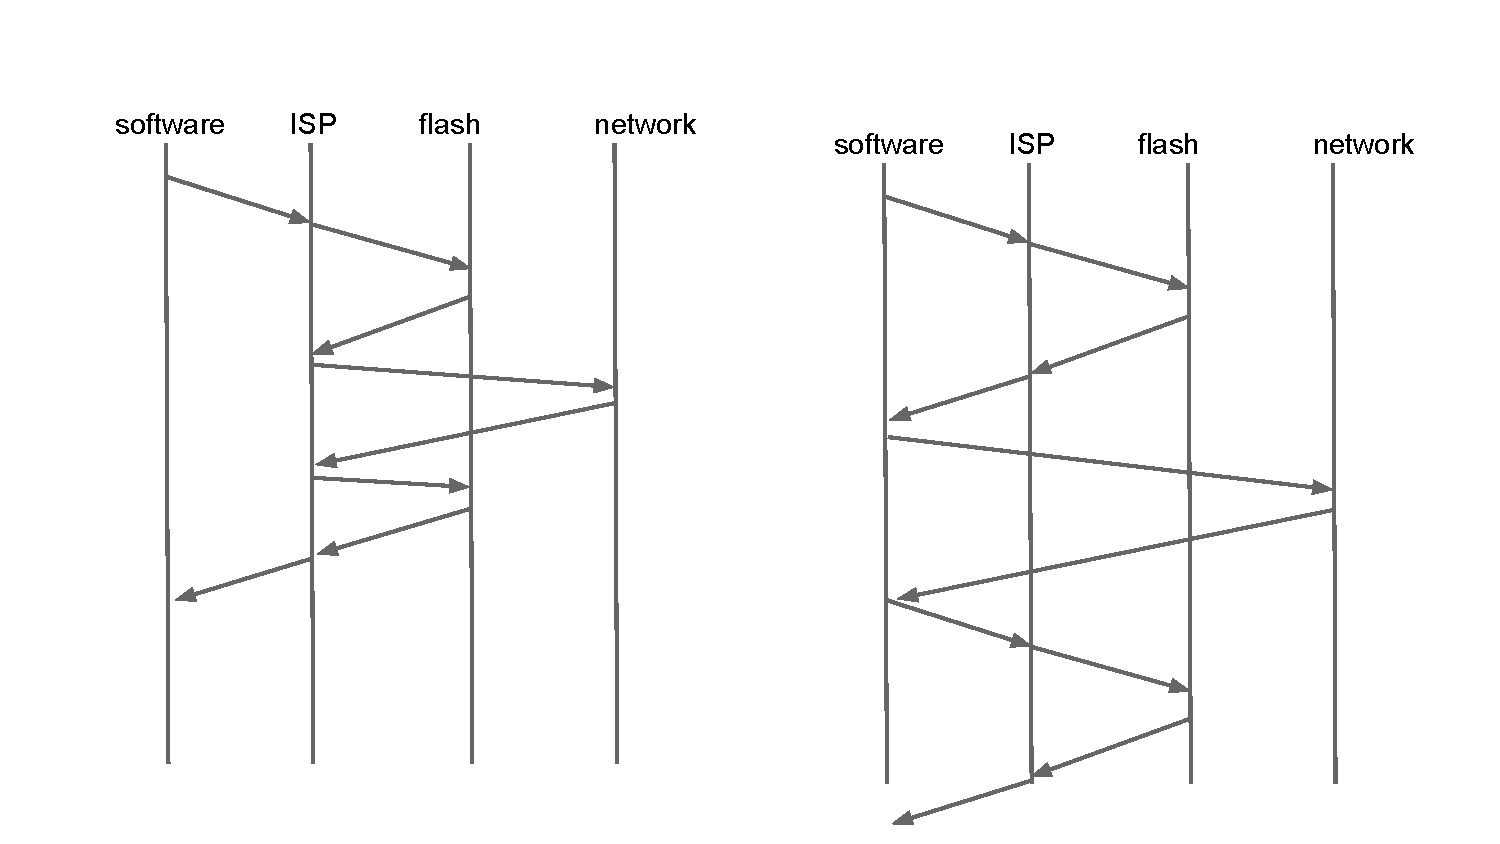
\includegraphics[width=0.4\paperwidth]{figures/graph_accel.pdf}
%	\caption{Graph Traversal Comparison}
%	\label{fig:graph_accel}
%	\end{center}
%\end{figure}

\begin{figure}[ht!]
	\centering
	\subfloat[Using ISP and Integrated Network]
		{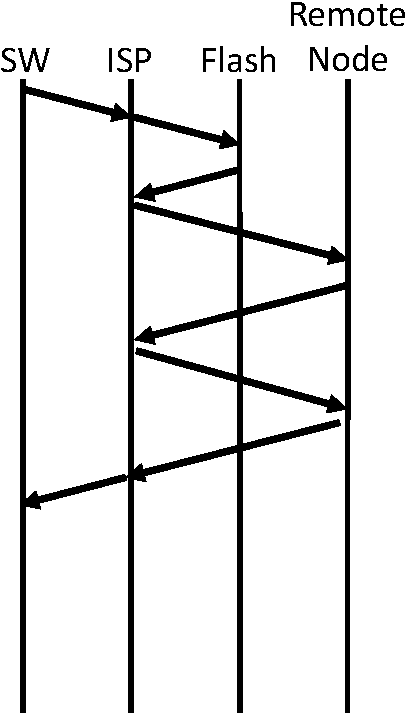
\includegraphics[width=0.18\textwidth]{figures/graph_isp-crop.pdf}}
		\hfill
	\subfloat[Using Software]
		{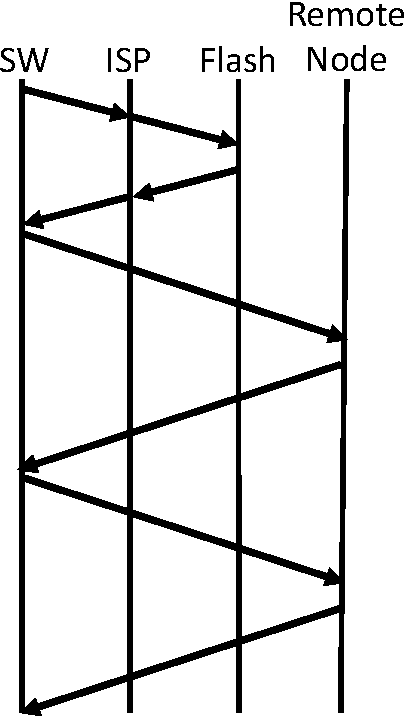
\includegraphics[width=0.18\textwidth]{figures/graph_sw-crop.pdf}}
		\hfill
	\caption{Graph Traversal Comparison}
	\label{fig:graph_accel}
\end{figure}

\subsection{String Search}

String search is common operation in analytics, often used in
database table scans, DNA sequence matching and cheminformatics. It is 
primarily a sequential read and compare workload. We
examine its performance on FlashBoost with assistance from in-store Morris-Pratt (MP) 
string search engines~\cite{?} fully integrated with the file system, flash controller
and application software.  The software portion of string search initially sets
up the accelerator by transferring the target string pattern (needle) and a set
of precomputed MP constants over DMA. Then it consults the file system for a
list of physical addresses of the files to search (haystack).  This list is
streamed to the accelerator, which uses these addresses to request for pages
from the flash controller.  The accelerated MP engines may operate in parallel
either by searching multiple files or by dividing up the haystack into equal
segments (with some overlaps). This choice depends on the number of files and
size of each file. Since 4 read commands can saturate a single flash bus, we
use 4 engines per bus to maximize the flash bandwidth. Only
search results are returned to the server. 
